\section{Results}
\label{sec:results}

\subsection{Line curvature and extraction}
Dispersion runs along $x$, blue to the left. The slit images are not straight but parabolic, with a sagitta of $\sim$\CurvSagitta~px between rows 250 and 800 and a mean tilt of \CurvTilt$^\circ$ in the extracted region. The quadratic trace fits the centroids with \CurvRMS~px rms and removes the curvature (Fig.~\ref{fig:curv}). The line width also changes along the slit (Fig.~\ref{fig:fwhmrow}): it is minimum, $\sim$3~px, in rows 450--550 and grows to 5--7~px towards the ends, so only that band was extracted.

\begin{figure}[htbp]
\centering
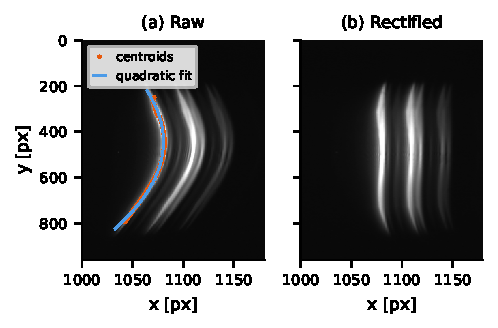
\includegraphics[width=\linewidth]{curvatura_lineas.pdf}
\caption{Kr lines around 760--830~nm. (a) Raw frame with the centroids of the traced line and the quadratic fit. (b) Same region after rectification.}
\label{fig:curv}
\end{figure}

\begin{figure}[htbp]
\centering
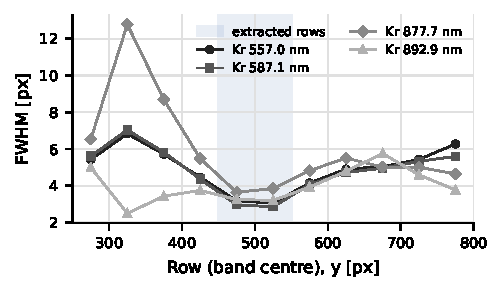
\includegraphics[width=\linewidth]{fwhm_vs_fila.pdf}
\caption{FWHM of four isolated Kr lines measured in 50-row bands along the slit. The shaded band marks the extracted rows.}
\label{fig:fwhmrow}
\end{figure}

\subsection{Line identification and wavelength calibration}
The lamps used were the following: the white lamp is krypton (weak lines at 557.0 and 587.1~nm, strong ones at 758--830~nm) and the rose one is argon (696.5, 706.7, 763.5, 811.5, 912.3, 965.8~nm). Fig.~\ref{fig:gauss} shows the profiles and Gaussian fits of all sources. The LEDs are 20--27~nm wide, far broader than the atomic lines, so they are used only as an independent check. Of the \NFeatures{} fitted lamp features, \CalN{} are isolated lines; the rest are unresolved blends and were not used.

\begin{figure*}[htbp]
\centering
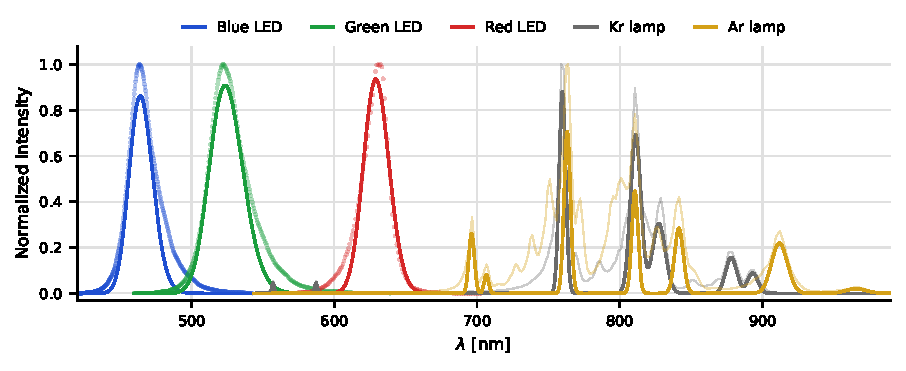
\includegraphics[width=\textwidth]{gaussianas_leds_lamparas.pdf}
\caption{Spectral profiles (faint) and Gaussian fits (solid) of the three LEDs and of the Kr and Ar lamps, normalized to the peak of each source and plotted with the final calibration.}
\label{fig:gauss}
\end{figure*}

The Hartmann fit to the \CalN{} isolated lines gives $\lambda_0=\HartLamZero$~nm, $C=$~\HartC~nm\,px and $x_0=\HartXzero$~px, with residuals of \CalRMS~nm rms (Fig.~\ref{fig:cal}, Table~\ref{tab:lines}). Applied to the LEDs, which were not in the fit, it places them at \LEDBlue, \LEDGreen{} and \LEDRed~nm (Table~\ref{tab:leds}), consistent with typical blue, green and red LEDs. This also checks the blue end, where the calibration is an extrapolation.

\begin{figure}[htbp]
\centering
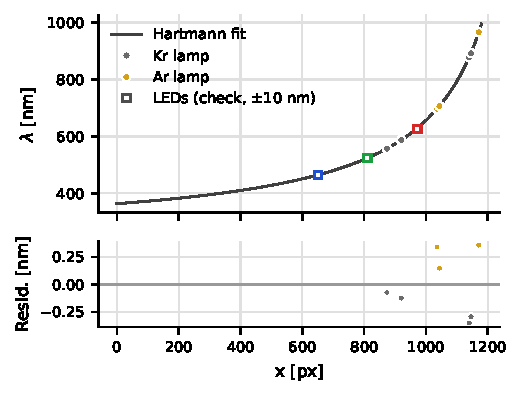
\includegraphics[width=\linewidth]{calibracion.pdf}
\caption{Hartmann calibration with the isolated Kr and Ar lines (top) and its residuals (bottom). The LEDs (squares, nominal $\lambda\pm10$~nm) are not part of the fit.}
\label{fig:cal}
\end{figure}

\begin{table}[htbp]
\caption{Isolated lines: laboratory wavelength [nm], centroid, calibration residual [nm], FWHM, reciprocal dispersion, resolution element and resolving power.}
\label{tab:lines}
\centering
\scriptsize
\setlength{\tabcolsep}{3pt}
\begin{tabular}{@{}lrrrrrrr@{}}
\toprule
Lamp & $\lambda_{\rm lab}$ & $x$ [px] & Resid. & FWHM [px] & $P$ [nm/px] & $\Delta\lambda$ [nm] & $R$ \\
\midrule
Kr & 557.0 & 873.7 & $-$0.07 & 3.1 & 0.59 & 1.9$\pm$0.1 & 301 \\
Kr & 587.1 & 920.0 & $-$0.13 & 2.9 & 0.71 & 2.1$\pm$0.1 & 283 \\
Ar & 696.5 & 1035.7 & +0.34 & 3.7 & 1.24 & 4.6$\pm$0.3 & 153 \\
Ar & 706.7 & 1043.8 & +0.15 & 2.8 & 1.30 & 3.7$\pm$0.8 & 191 \\
Kr & 877.7 & 1139.7 & $-$0.35 & 3.8 & 2.45 & 9.2$\pm$0.4 & 95 \\
Kr & 892.9 & 1145.8 & $-$0.29 & 3.2 & 2.57 & 8.3$\pm$0.7 & 107 \\
Ar & 965.8 & 1171.0 & +0.36 & 5.3 & 3.18 & 16.8$\pm$0.8 & 58 \\
\bottomrule
\end{tabular}

\end{table}

\begin{table}[htbp]
\caption{LED positions from the calibration (fit error only).}
\label{tab:leds}
\centering
\footnotesize
\begin{tabular}{@{}lccc@{}}
\toprule
Source & $\lambda_{\rm nom}$ & $\lambda_{\rm meas}$ [nm] & FWHM [nm] \\
\midrule
Blue LED & 465 & 464.2$\pm$0.6 & 19.4 \\
Green LED & 525 & 523.6$\pm$0.4 & 27.4 \\
Red LED & 625 & 629.2$\pm$0.2 & 21.1 \\
\bottomrule
\end{tabular}

\end{table}

\subsection{Dispersion}
The measured reciprocal dispersion is the derivative of the calibration, $P=|C|/(x-x_0)^2$ (Fig.~\ref{fig:disp}). It grows from \DispMeasFiveH~nm/px at 500~nm to \DispMeasSixH~nm/px at 600~nm and \DispMeasEightH~nm/px at 800~nm. Its shape follows the SF18 prism (the ratio to the model varies only \DispRatioSpread\% over 440--970~nm), but its value is \DispRatio{} times the design one: the spectrum is more compressed than expected, maybe due to the camera being at 27~mm instead of 40~mm.

\begin{figure}[htbp]
\centering
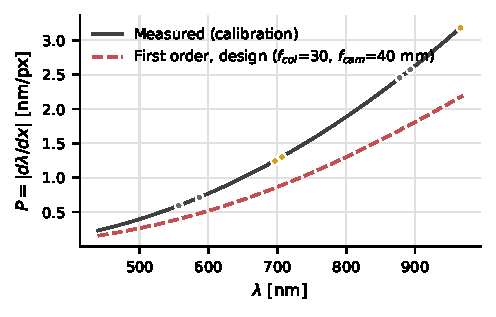
\includegraphics[width=\linewidth]{dispersion.pdf}
\caption{Measured reciprocal dispersion (derivative of the calibration; dots at the calibration lines) and first-order design value.}
\label{fig:disp}
\end{figure}

\subsection{Resolution}
The isolated Kr lines have a median FWHM of \FWHMKr~px and the Ar lines \FWHMAr~px. The resolution element grows from about 2~nm at 557--587~nm to 17~nm at 966~nm, and the resolving power falls from $R\approx\RMax$ to $R\approx\RMin$ (Table~\ref{tab:lines}, Fig.~\ref{fig:res}). The measured values are above the design curve at all wavelengths covered by Kr.

\begin{figure}[htbp]
\centering
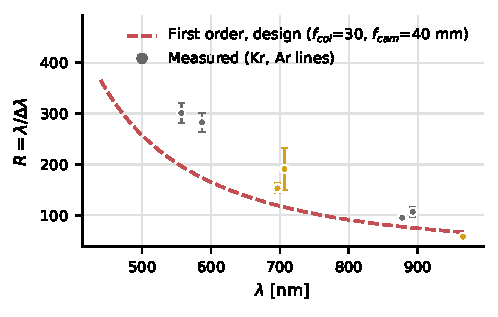
\includegraphics[width=\linewidth]{resolucion.pdf}
\caption{Measured resolving power (Kr grey, Ar yellow) and first-order design value for a \SI{25}{\micro\meter} slit.}
\label{fig:res}
\end{figure}

\subsection{Spectral range}
\label{sec:range}
The flash spectrum (Fig.~\ref{fig:flash}) shows the pump LED peak near 450~nm, the dip near 480~nm and the broad phosphor band. With a \RangeThr\% threshold the range is \RangeMin--\RangeMax~nm. \FlashSat\% of the flash pixels are saturated, which flattens 520--610~nm. The calibration places the blue edge of the detector ($x=0$) at \RangeDetMin~nm, and the Ar line at \RangeLastLine~nm was detected at the red end, so the instrument covers at least \RangeDetMin--\RangeLastLine~nm and the flash range is set by the source.

\begin{figure}[htbp]
\centering
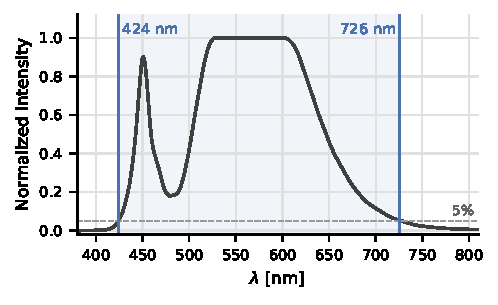
\includegraphics[width=\linewidth]{flash_rango.pdf}
\caption{Phone flash spectrum and range defined at \RangeThr\% of the peak.}
\label{fig:flash}
\end{figure}

\begin{table}[htbp]
\caption{Summary: first-order design vs.\ measured values.}
\label{tab:summary}
\centering
\footnotesize
\begin{tabular}{@{}lcc@{}}
\toprule
Parameter & Design & Measured \\
\midrule
$P$ at 500 nm [nm/px] & 0.26 & 0.39 \\
$P$ at 600 nm [nm/px] & 0.52 & 0.77 \\
$P$ at 800 nm [nm/px] & 1.30 & 1.88 \\
Slit image FWHM [px] & 7.2 & 3.2 \\
$\Delta\lambda$ at 557 nm [nm] & 2.8 & 1.9 \\
$R$ at 557 nm & 197 & 301 \\
$R$ at 878 nm & 77 & 95 \\
Range [nm] & 416--$>$1000$^a$ & 424--726$^b$ \\
\bottomrule
\end{tabular}
\\[2pt]
\parbox{0.95\linewidth}{\scriptsize $^a$Detector limit with 550~nm centred. $^b$Flash, limited by the source; detector covers at least \RangeDetMin--\RangeLastLine~nm.}
\end{table}
